% This is a sample document using the University of Minnesota, Morris, Computer Science
% Senior Seminar modification of the ACM sig-alternate style. Much of this content is taken
% directly from the ACM sample document illustrating the use of the sig-alternate class. Certain
% parts that we never use have been removed to simplify the example, and a few additional
% components have been added.

% See https://github.com/UMM-CSci/Senior_seminar_templates for more info and to make
% suggestions and corrections.

\documentclass{sig-alternate}
\usepackage{color}

\setlength{\marginparwidth}{2cm}
\usepackage[colorinlistoftodos]{todonotes}

\usepackage{url}

%%%%% Uncomment the following line and comment out the previous one
%%%%% to remove all comments
%%%%% NOTE: comments still occupy a line even if invisible;
%%%%% Don't write them as a separate paragraph
%\newcommand{\mycomment}[1]{}

\begin{document}

% --- Author Metadata here ---
%%% REMEMBER TO CHANGE THE SEMESTER AND YEAR AS NEEDED
\conferenceinfo{UMM CSci Senior Seminar Conference, October 2020}{Morris, MN}

\title{Recent advances in smartphone computational photography}

\numberofauthors{1}

\author{
% The command \alignauthor (no curly braces needed) should
% precede each author name, affiliation/snail-mail address and
% e-mail address. Additionally, tag each line of
% affiliation/address with \affaddr, and tag the
% e-mail address with \email.
\alignauthor
Paul Friederichsen\\
	\affaddr{Division of Science and Mathematics}\\
	\affaddr{University of Minnesota, Morris}\\
	\affaddr{Morris, Minnesota, USA 56267}\\
	\email{fried701@morris.umn.edu}
}

\maketitle

\begin{abstract}
(This is currently just a topic statement more than an abstract)

My topic is recent advances in the computational photography used in smartphones. Specifically looking at the use of multi-frame algorithms to increase image resolution and quality. I'm mainly looking at a couple of papers by researchers at Google on algorithms used in the Super-Res Zoom and Night Sight features of the Google Pixel series of smartphones.
\end{abstract}

\keywords{computational photography, super-resolution, image processing, low-light imaging}

\section{Introduction}

Smartphone cameras present many challenges, most of which come from the need for them to be physically small. Their small size puts a fundamental limit on their ability to resolve detail and especially affects low-light photography. This paper will look at two approaches to improve smartphone photography through software techniques.

% ----------------------------------------
\section{Background}

\subsection{Burst photography}

Most smartphones use a burst processing pipeline for their cameras. Generally, burst processing involves taking a series of raw exposures and merging them together to form the final image. Most smartphones operate in a \emph{Zero-Shutter Lag} mode by default. In this mode raw frames are continuously captured to a ring buffer while the camera app is open. When the user presses the shutter button, a number of the most recent frames are sent to the camera processing pipeline.

Both of the approaches in this paper build on the end-to-end burst processing pipeline from Hasinoff et al. \cite{Hasinoff2016} which used bursts of constant low-exposure frames to increase dynamic range and signal-to-noise ratio.
% TODO: more on Hasinoff

\newpage

\subsection{Bayer filter}

The majority of digital image sensors in digital cameras and phones use a Bayer filter mosaic pattern to arrange RGB color filters on the sensor. The pattern consists of 50\% green, 25\% red, and 25\% blue pixels \cite{wiki:BayerFilter}. This ratio emulates the color sensitivity of the human eye. Due to this pattern on the sensor, the raw output of a digital camera also has each pixel filtered to only red, green, or blue and a demosaicing algorithm must be used to interpolate the other values for each pixel \cite{wiki:BayerFilter}.

\begin{figure}
\centering
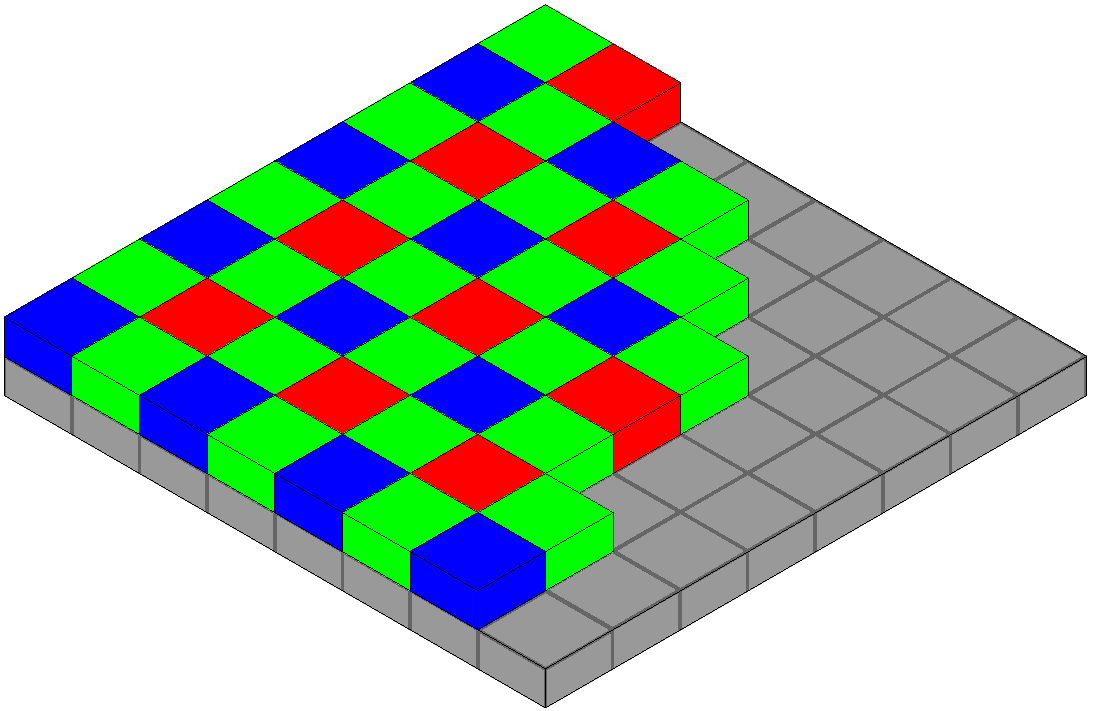
\psfig{file=figures/Bayer_pattern_on_sensor.pdf,width =3in}
\caption{A Bayer pattern on a sensor in isometric perspective \cite{wiki:BayerFilter}.}
\label{fig:BayerPattern}
\end{figure}

\subsection{Demosaicing}

Background information on demosaicing. Some of this will come from \cite{wiki:Demosaicing}.

The demosaicing process may introduce various artifacts in the final image. These typically include false color artifacts like zippering and Moiré patterns \cite{Wronski2019}.

\subsection{Aliasing}

Background information on aliasing, specifically in regard to signal processing. Some of this will come from \cite{wiki:Aliasing}.

\subsection{Super-resolution}

% ----------------------------------------
\section{Handheld super-resolution}

\begin{figure*}[t!]
\centering
% TODO: Size correctly for width
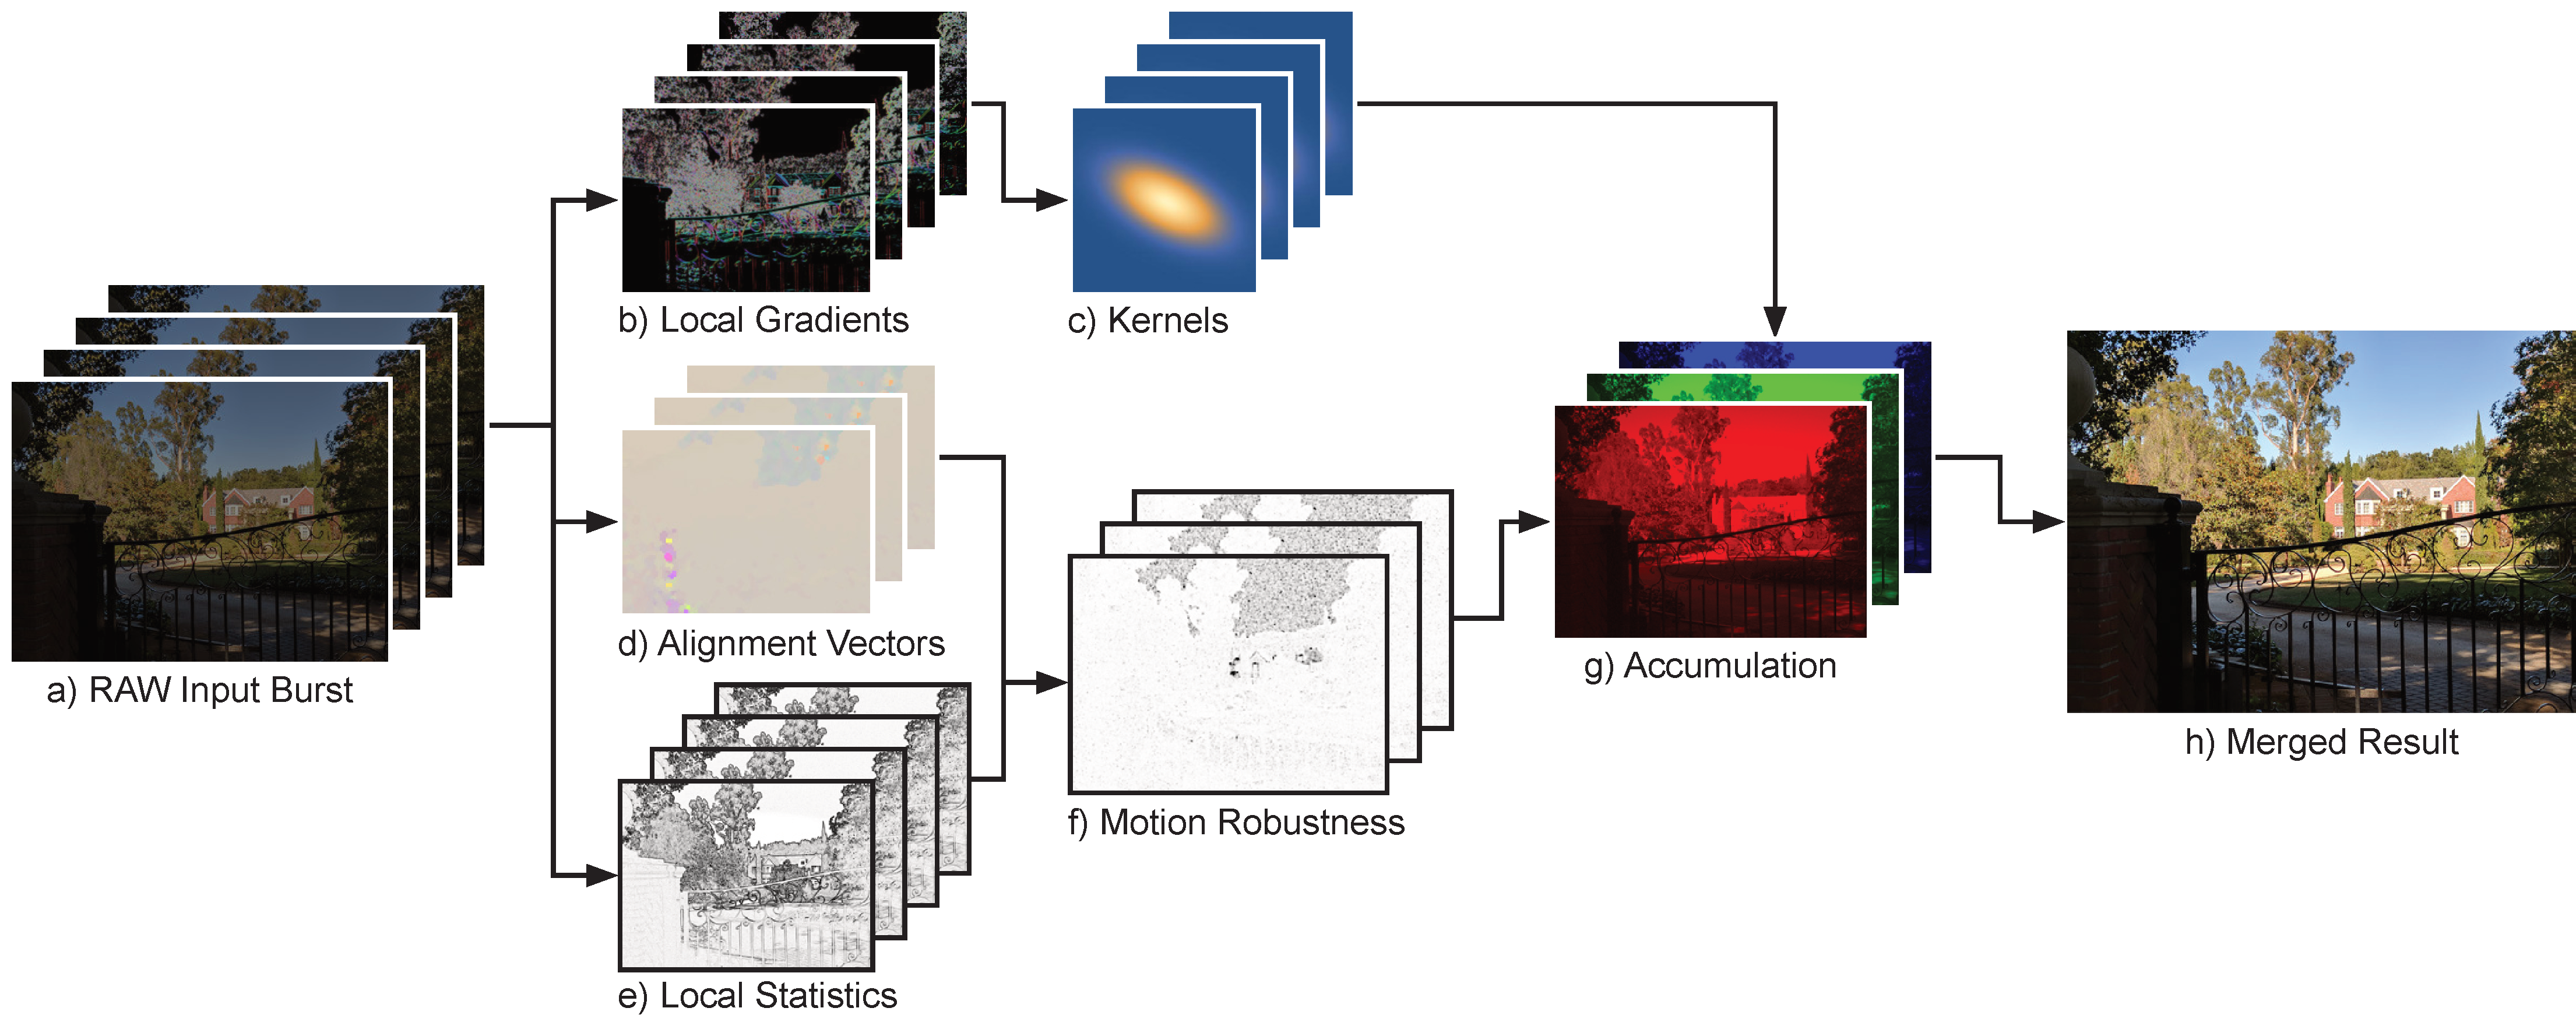
\psfig{file=figures/Wronski2019-figure-2.pdf,width =7in}
\caption{An overview of the approach used by Wronski et al. \cite{Wronski2019}}
\label{fig:Wronski2019Fig2}
\end{figure*}

Wronski et al.~\cite{Wronski2019} introduce an algorithm that uses multiple shifted frames to produce higher resolution images from bursts of underexposed raw frames as part of the smartphone's imaging pipeline. The algorithm is able to directly use Bayer raw frames and removes the need for an explicit demosaicing step in the pipeline. It uses natural hand motion and is efficient enough to work in the background on smartphones.

\subsection{Algorithm overview}

Wronski et al.'s approach is a process that starts with the the acquisition of a burst from the continous ring buffer of raw frames in the phone's camera application. Next, a single frame is chosen and the rest are aligned to it using a refined version of the algorithm by Hasinoff et al.~\cite{Hasinoff2016}.
% TODO: elaborate on the alignment algorithm
Each frame's local contributions are estimated through kernel regression (Section~\ref{sec:kernelReconstruction}) and accumulated across an whole burst for each of the three color planes.
Next, in parallel, the kernel shapes are adjusted based on estimated local gradients and the sample contributions are adjusted weighted based on a robustness model (Section~\ref{sec:robustnessModel}).
The final RGB image is obtained by normalizing the accumulated contributions for each of the three color planes and merging them together.

\subsection{Hand movement based super-resolution}

One of the important conditions for multi-frame super-resolution is that the input contains multiple aliased images that are sampled at different subpixel offsets. When someone is holding an object there is a natural and involuntary slight hand movement present. Wronski et al. shows how this periodic, random movement while the camera is capturing a burst frames provides sufficient subpixel coverage to create a super-resolution image.

Wronski et al. analyzed hand movement in a set of 86 bursts captured by 10 different users during regular smartphone photography. They used the rotational measurements from the phone's gyroscope but ignored the effect of translations in the analysis. Their analysis showed that hand movement creates uniformly random angular displacements and relatively slow rotation of the device.


While hand shake over a long time interval uniformly random, over a short burst it could be more of a straight line.
Wronski et al. show that this also provides a sufficiently uniform distribution of subpixel samples.
Using the equidistribution theorem, which states that the sequence $\{a,2a,3a,\dotsc \bmod 1\}$ is uniformly distributed (assuming $a$ is an irrational number), with each pixel as a point sample and a least random scenario (the hand motion is regular and linear), the samples from all frames combined will be approximately uniformly distributed within the subpixel space.

Wronski et al. also tested this concept empirically by measuring subpixel offsets by registration across 20 handheld bursts. They found some deviation from a uniform distribution largely caused by pixel locking, which causes a bias towards whole pixel values. Overall, the subpixel coverage remained sufficient to be used for super-resolution.

\subsection{Proposed super-resolution approach}

\subsubsection{Kernel reconstruction}
\label{sec:kernelReconstruction}

\subsubsection{Motion Robustness}
\label{sec:robustnessModel}

\subsection{Results}

\subsubsection{Limitations}

% ----------------------------------------
\section{Handheld low light photography}



\subsection{Motion Metering}


\subsection{Motion-adaptive burst merging}


\subsection{Auto white balance in low-light}



\subsection{Tone mapping}


\subsection{Results}


\subsubsection{Limitations}

% ----------------------------------------
\section{Conclusions}



\section*{Acknowledgments}
\label{sec:acknowledgments}


% The following two commands are all you need in the
% initial runs of your .tex file to
% produce the bibliography for the citations in your paper.
\bibliographystyle{abbrv}
% sample_paper.bib is the name of the BibTex file containing the
% bibliography entries. Note that you *don't* include the .bib ending here.
\bibliography{paper}  
% You must have a proper ".bib" file
%  and remember to run:
% latex bibtex latex latex
% to resolve all references

\end{document}